\documentclass{beamer}
\usepackage{epstopdf}
\usepackage{amsfonts}
\usepackage{amsmath}
\usepackage{graphicx}
\usepackage{subfigure}
\usepackage{siunitx}
\usepackage{todonotes}
\usepackage{booktabs}
\usepackage{color, colortbl}
\definecolor{Gray}{gray}{0.95}

\providecommand{\e}[1]{\ensuremath{\times 10^{#1}}}
\providecommand{\m}[1]{\ensuremath{\mathrm{#1}}}
\providecommand{\p}[1]{\ensuremath{\partial #1}}

\newcommand{\figWidth}{0.5\textwidth}
\newcommand{\subfigWidth}{0.45\textwidth}
\graphicspath{{figs/}} 


\usetheme{Boadilla}
%\usetheme{CambridgeUS}
%\usetheme{boxes}


\begin{document}


\begin{frame}{Outline}
\begin{enumerate}
 \item Biological background
 \item Bolie's glucose-insulin interaction model and it's linearization
 \item Bellomo's model
 \item Diagnosing diabetes
\end{enumerate}


\end{frame}

% Jachymovy slajdy ----------
\begin{frame}{Biological facts and assumptions}
\begin{enumerate}
	\item
	Insulin is being degraded by the liver.	
	\item
	A rise in the concentration of glucose in the bloodstream results in increased production of insulin by the pancreas.
	\item
	With increasing concentration of insulin, the glucose is more easily absorbed by the cells, i.e. it leaves the bloodstream more quickly.
	\item
	A rise in glucose concentration in the bloodstream results in increased glucose absorption by the liver.

\end{enumerate}
\end{frame}

% Jiriho slajdy ----------
\begin{frame}{Bolie's glucose-insulin interaction model (1)}

\begin{enumerate}
	\item
	Insulin is being degraded by the liver.	
	\item
	More glucose in the bloodstream results in faster production of insulin.
\end{enumerate}

\begin{align*}
\underbrace{V}_%
{\text{liter}}%
%
\underbrace{\frac{\m{d} H}{\m{d} t}}_%
{\frac{\text{unit}}{\text{liter} \times\text{hour}}}
=%
\underbrace{-F_1(H)+F_2(G)+\text{insulin injection rate}}%
_{\frac{\text{unit}}{\text{hour}}}
\end{align*}

\end{frame}

\begin{frame}{Bolie's glucose-insulin interaction model (2)}

\begin{enumerate}
\setcounter{enumi}{2}
	\item
	With more insulin, glucose disappears from the bloodstream more quickly. 
	\item
	Glucose is degraded more quickly when more concentrated
\end{enumerate}

\begin{align*}
\underbrace{V}_%
{\text{liter}}%
%
\underbrace{\frac{\m{d} G}{\m{d} t}}_%
{\frac{\text{gram}}{\text{liter} \times\text{hour}}}
=%
\underbrace{-F_3(H,G)-F_4(H,G) +\text{glucose injection rate}}%
_{\frac{\text{gram}}{\text{hour}}}
\end{align*}


\end{frame}

\begin{frame}{Bolie's model for small changes around equilibrium}
\centering{Equilibrium of insulin and glucose in the bloodstream\\ $(H_0$, $G_0)=(\mathbf{e}_0)$} 

\begin{equation*}
\begin{aligned}
V\frac{\m{d}h}{\m{d}t}&=-F_1(H_0+h)+F_2(G_0+g)+ \text{insulin injection rate},\\
V\frac{\m{d}g}{\m{d}t}&=-F_3(H_0+h,G_0+g)-F_4(H_0+h,G_0+g)+ \text{g. injection rate}.
\end{aligned}
\end{equation*}
\end{frame}

\begin{frame}{Linearization of Bolie's model}

\centering{Equilibrium of insulin and glucose in the bloodstream\\ $(H_0$, $G_0)=(\mathbf{e}_0)$} 

\begin{align*}
\frac{\m{d}h}{\m{d}t}&=-\underbrace{%
		\frac{1}{V}\frac{\p F_1(H_0)}{\p H}}_{\alpha}h+%
%
\underbrace{%
		\frac{1}{V}\frac{\p F_2(G_0)}{\p G}}_{\beta}g+\mathcal{O}(2), \\%		
%
\frac{\m{d}g}{\m{d}t}&=%
%
-\underbrace{%
\frac{1}{V}\left(\frac{\p F_3(\mathbf{e}_0)}{\p H}+\frac{\p F_4(\mathbf{e}_0)}{\p H}\right)}_{\gamma}h%
-\underbrace{%
\frac{1}{V}\left(\frac{\p F_3(\mathbf{e}_0)}{\p G}+\frac{\p F_4(\mathbf{e}_0)}{\p G}\right)}_{\delta} g+\mathcal{O}(2).
\end{align*}


\end{frame}

\begin{frame}{Linearized Bolie's model}

System of 1\textsuperscript{st} order equations
\begin{equation*}
\begin{aligned}
\frac{\m{d}h}{\m{d}t}&=-\alpha h + \beta g,\\
\frac{\m{d}g}{\m{d}t}&=-\gamma h - \delta g.\\
\end{aligned}
\end{equation*}

Reduced 2\textsuperscript{nd} order equation
\begin{equation*}
	\ddot g+\underbrace{%
	(\gamma+\beta)}%
	_{- \text{trace }> \,0}%
	\dot g+\underbrace{%
	(\beta \gamma+\delta \alpha)}%
	_{\text{determinant }> \,0}g=0.
\end{equation*}

%Eigenvalues and general solution
%\begin{equation*}
%	\lambda_{1,2}=\frac{1}{2}\left(-(\gamma+\beta)\pm \sqrt{(\gamma+\beta)^2-4(\beta\gamma+\delta\alpha)}\right).
%\end{equation*}
%
%\begin{equation*}
%	g(t) = A\,e^{\lambda_1 \, t} + B\,e^{\lambda_2 \, t}.
%\end{equation*}

\end{frame}

%\begin{frame}{Initial conditions response of the Bolie's model}
%\begin{equation*}
%	\ddot g+(\gamma+\beta)\dot g+(\beta \gamma+\delta \alpha)g=0.
%\end{equation*}\\
%\vspace{1cm}
%What happens according to the model when a patient gets a dose of glucose?\\
%
%\centering{$g(t_0=0) = g_0\,$ and $\,h(t_0=0)=0$}
%
%\begin{equation*}
%\dot g=-\gamma h - \delta g \quad \Rightarrow \quad h = -\frac{1}{\gamma}\left( \dot{g} + \delta\,g \right) \quad \Rightarrow  \quad \dot g(t_0=0)=-\delta g_0
%\end{equation*}
%
%\begin{equation*}	
%	A = g_0\,\frac{\delta+\lambda_2}{\lambda_2-\lambda_1}, \qquad B = g_0\,\frac{\delta+\lambda_1}{\lambda_1-\lambda_2}.
%\end{equation*}
%
%
%\end{frame}

% Opět Jáchymovy slajdy
\begin{frame}{Bellomo's model}
A special case of the general Bolie's model
\begin{align*}
 \frac{\m{d}i}{\m{d}t} &= -\underbrace{K_{\mathrm{i}}\,i}_{F_1} + \underbrace{K_{\mathrm{g}}\,(g - g_{\mathrm{d}})}_{F_2} + \underbrace{K_{\mathrm{s}}\,i_{\mathrm{r}}}_{x}, \\
 \frac{\m{d}g}{\m{d}t} &= \underbrace{K_{\mathrm{h}}\,g - K_0\,g\,i - K_{\mathrm{s}}\,K_{\mathrm{f}}}_{-F_3-F_4} + \underbrace{0}_{y}.
\end{align*}
How do we interpret the terms $K_{\mathrm{h}}\,g - K_0\,g\,i - K_{\mathrm{s}}\,K_{\mathrm{f}}$?
\[ K_{\mathrm{h}}\,g - K_0\,g\,i = K_{\mathrm{n}}\,g\left(1 - \frac{K_0}{K_{\mathrm{n}}}\,i\right) := K_{\mathrm{n}}\,g(1 - a\,i). \]

\end{frame}

% Martinovy slajdy ----------
\begin{frame}{Ackerman's diabetes test}

\begin{equation*}
	\label{Eq:GT}
	G(t) = G_0 + C\,e^{-\sigma t}\cos ( \omega t  - \varphi)
\end{equation*}

\begin{figure}[h!t!]
   \centering
   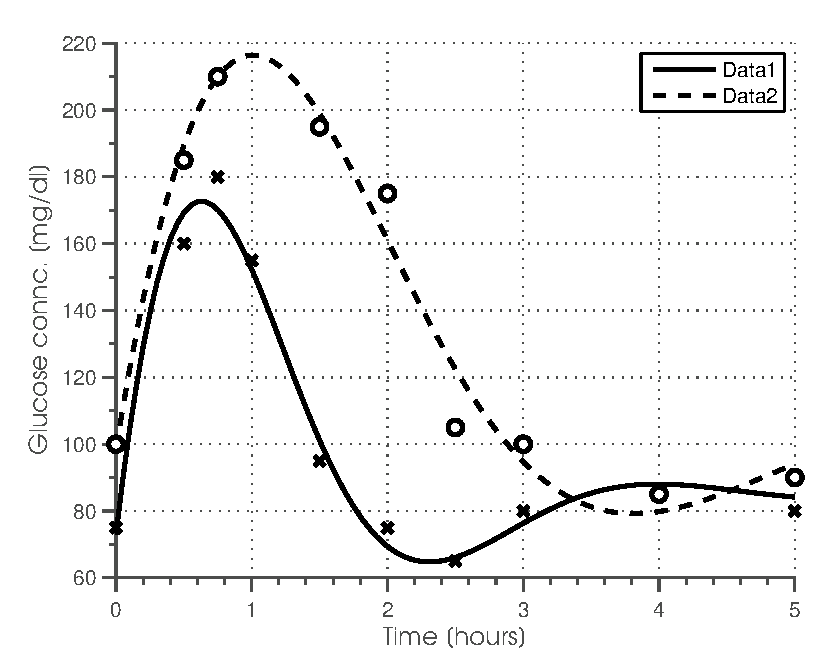
\includegraphics[width=0.7\textwidth]{figs/ackermanTestPres}
\end{figure}
\end{frame}

\begin{frame}{Bolie's diabetes test}
\begin{figure}[h!t!]
   \centering
   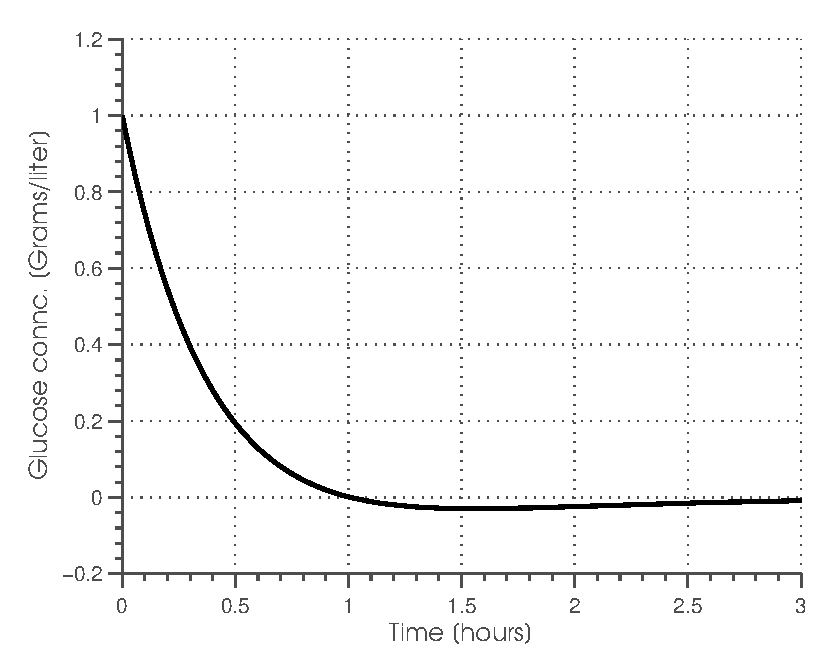
\includegraphics[width=0.7\textwidth]{figs/boliesTestGlucosePres}
\end{figure}
\end{frame}

\end{document}
